\documentclass[]{book}
\usepackage{lmodern}
\usepackage{amssymb,amsmath}
\usepackage{ifxetex,ifluatex}
\usepackage{fixltx2e} % provides \textsubscript
\ifnum 0\ifxetex 1\fi\ifluatex 1\fi=0 % if pdftex
  \usepackage[T1]{fontenc}
  \usepackage[utf8]{inputenc}
\else % if luatex or xelatex
  \ifxetex
    \usepackage{mathspec}
  \else
    \usepackage{fontspec}
  \fi
  \defaultfontfeatures{Ligatures=TeX,Scale=MatchLowercase}
\fi
% use upquote if available, for straight quotes in verbatim environments
\IfFileExists{upquote.sty}{\usepackage{upquote}}{}
% use microtype if available
\IfFileExists{microtype.sty}{%
\usepackage{microtype}
\UseMicrotypeSet[protrusion]{basicmath} % disable protrusion for tt fonts
}{}
\usepackage[margin=1in]{geometry}
\usepackage{hyperref}
\hypersetup{unicode=true,
            pdftitle={Linear Regression 303},
            pdfauthor={Alfonso R. Reyes},
            pdfborder={0 0 0},
            breaklinks=true}
\urlstyle{same}  % don't use monospace font for urls
\usepackage{natbib}
\bibliographystyle{apalike}
\usepackage{color}
\usepackage{fancyvrb}
\newcommand{\VerbBar}{|}
\newcommand{\VERB}{\Verb[commandchars=\\\{\}]}
\DefineVerbatimEnvironment{Highlighting}{Verbatim}{commandchars=\\\{\}}
% Add ',fontsize=\small' for more characters per line
\usepackage{framed}
\definecolor{shadecolor}{RGB}{248,248,248}
\newenvironment{Shaded}{\begin{snugshade}}{\end{snugshade}}
\newcommand{\AlertTok}[1]{\textcolor[rgb]{0.94,0.16,0.16}{#1}}
\newcommand{\AnnotationTok}[1]{\textcolor[rgb]{0.56,0.35,0.01}{\textbf{\textit{#1}}}}
\newcommand{\AttributeTok}[1]{\textcolor[rgb]{0.77,0.63,0.00}{#1}}
\newcommand{\BaseNTok}[1]{\textcolor[rgb]{0.00,0.00,0.81}{#1}}
\newcommand{\BuiltInTok}[1]{#1}
\newcommand{\CharTok}[1]{\textcolor[rgb]{0.31,0.60,0.02}{#1}}
\newcommand{\CommentTok}[1]{\textcolor[rgb]{0.56,0.35,0.01}{\textit{#1}}}
\newcommand{\CommentVarTok}[1]{\textcolor[rgb]{0.56,0.35,0.01}{\textbf{\textit{#1}}}}
\newcommand{\ConstantTok}[1]{\textcolor[rgb]{0.00,0.00,0.00}{#1}}
\newcommand{\ControlFlowTok}[1]{\textcolor[rgb]{0.13,0.29,0.53}{\textbf{#1}}}
\newcommand{\DataTypeTok}[1]{\textcolor[rgb]{0.13,0.29,0.53}{#1}}
\newcommand{\DecValTok}[1]{\textcolor[rgb]{0.00,0.00,0.81}{#1}}
\newcommand{\DocumentationTok}[1]{\textcolor[rgb]{0.56,0.35,0.01}{\textbf{\textit{#1}}}}
\newcommand{\ErrorTok}[1]{\textcolor[rgb]{0.64,0.00,0.00}{\textbf{#1}}}
\newcommand{\ExtensionTok}[1]{#1}
\newcommand{\FloatTok}[1]{\textcolor[rgb]{0.00,0.00,0.81}{#1}}
\newcommand{\FunctionTok}[1]{\textcolor[rgb]{0.00,0.00,0.00}{#1}}
\newcommand{\ImportTok}[1]{#1}
\newcommand{\InformationTok}[1]{\textcolor[rgb]{0.56,0.35,0.01}{\textbf{\textit{#1}}}}
\newcommand{\KeywordTok}[1]{\textcolor[rgb]{0.13,0.29,0.53}{\textbf{#1}}}
\newcommand{\NormalTok}[1]{#1}
\newcommand{\OperatorTok}[1]{\textcolor[rgb]{0.81,0.36,0.00}{\textbf{#1}}}
\newcommand{\OtherTok}[1]{\textcolor[rgb]{0.56,0.35,0.01}{#1}}
\newcommand{\PreprocessorTok}[1]{\textcolor[rgb]{0.56,0.35,0.01}{\textit{#1}}}
\newcommand{\RegionMarkerTok}[1]{#1}
\newcommand{\SpecialCharTok}[1]{\textcolor[rgb]{0.00,0.00,0.00}{#1}}
\newcommand{\SpecialStringTok}[1]{\textcolor[rgb]{0.31,0.60,0.02}{#1}}
\newcommand{\StringTok}[1]{\textcolor[rgb]{0.31,0.60,0.02}{#1}}
\newcommand{\VariableTok}[1]{\textcolor[rgb]{0.00,0.00,0.00}{#1}}
\newcommand{\VerbatimStringTok}[1]{\textcolor[rgb]{0.31,0.60,0.02}{#1}}
\newcommand{\WarningTok}[1]{\textcolor[rgb]{0.56,0.35,0.01}{\textbf{\textit{#1}}}}
\usepackage{longtable,booktabs}
\usepackage{graphicx,grffile}
\makeatletter
\def\maxwidth{\ifdim\Gin@nat@width>\linewidth\linewidth\else\Gin@nat@width\fi}
\def\maxheight{\ifdim\Gin@nat@height>\textheight\textheight\else\Gin@nat@height\fi}
\makeatother
% Scale images if necessary, so that they will not overflow the page
% margins by default, and it is still possible to overwrite the defaults
% using explicit options in \includegraphics[width, height, ...]{}
\setkeys{Gin}{width=\maxwidth,height=\maxheight,keepaspectratio}
\IfFileExists{parskip.sty}{%
\usepackage{parskip}
}{% else
\setlength{\parindent}{0pt}
\setlength{\parskip}{6pt plus 2pt minus 1pt}
}
\setlength{\emergencystretch}{3em}  % prevent overfull lines
\providecommand{\tightlist}{%
  \setlength{\itemsep}{0pt}\setlength{\parskip}{0pt}}
\setcounter{secnumdepth}{5}
% Redefines (sub)paragraphs to behave more like sections
\ifx\paragraph\undefined\else
\let\oldparagraph\paragraph
\renewcommand{\paragraph}[1]{\oldparagraph{#1}\mbox{}}
\fi
\ifx\subparagraph\undefined\else
\let\oldsubparagraph\subparagraph
\renewcommand{\subparagraph}[1]{\oldsubparagraph{#1}\mbox{}}
\fi

%%% Use protect on footnotes to avoid problems with footnotes in titles
\let\rmarkdownfootnote\footnote%
\def\footnote{\protect\rmarkdownfootnote}

%%% Change title format to be more compact
\usepackage{titling}

% Create subtitle command for use in maketitle
\providecommand{\subtitle}[1]{
  \posttitle{
    \begin{center}\large#1\end{center}
    }
}

\setlength{\droptitle}{-2em}

  \title{Linear Regression 303}
    \pretitle{\vspace{\droptitle}\centering\huge}
  \posttitle{\par}
    \author{Alfonso R. Reyes}
    \preauthor{\centering\large\emph}
  \postauthor{\par}
      \predate{\centering\large\emph}
  \postdate{\par}
    \date{2019-09-18}

\usepackage{booktabs}

\begin{document}
\maketitle

{
\setcounter{tocdepth}{1}
\tableofcontents
}
\hypertarget{prerequisites}{%
\chapter*{Prerequisites}\label{prerequisites}}
\addcontentsline{toc}{chapter}{Prerequisites}

This is a \emph{sample} book written in \textbf{Markdown}. You can use anything that Pandoc's Markdown supports, e.g., a math equation \(a^2 + b^2 = c^2\).

The \textbf{bookdown} package can be installed from CRAN or Github:

\begin{Shaded}
\begin{Highlighting}[]
\KeywordTok{install.packages}\NormalTok{(}\StringTok{"bookdown"}\NormalTok{)}
\CommentTok{# or the development version}
\CommentTok{# devtools::install_github("rstudio/bookdown")}
\end{Highlighting}
\end{Shaded}

Remember each Rmd file contains one and only one chapter, and a chapter is defined by the first-level heading \texttt{\#}.

To compile this example to PDF, you need XeLaTeX. You are recommended to install TinyTeX (which includes XeLaTeX): \url{https://yihui.name/tinytex/}.

\hypertarget{generalised-additive-models-gams-an-introduction}{%
\chapter{Generalised additive models (GAMs): an introduction}\label{generalised-additive-models-gams-an-introduction}}

\hypertarget{introduction}{%
\section{Introduction}\label{introduction}}

Source: \url{http://environmentalcomputing.net/intro-to-gams/}

Many data in the environmental sciences do not fit simple linear models and are best described by ``wiggly models'', also known as Generalised Additive Models (GAMs).

Let's start with a famous tweet by one Gavin Simpson, which amounts to:

\begin{enumerate}
\def\labelenumi{\arabic{enumi}.}
\tightlist
\item
  GAMs are just GLMs
\item
  GAMs fit wiggly terms
\item
  use \texttt{+\ s(x)} not \texttt{x} in your syntax
\item
  use method \texttt{=\ "REML"}
\item
  always look at \texttt{gam.check()}
\end{enumerate}

This is basically all there is too it - an extension of generalised linear models (GLMs) with a smoothing function. Of course, there may be many sophisticated things going on when you fit a model with smooth terms, but you only need to understand the rationale and some basic theory. There are also lots of what would be apparently magic things happening when we try to understand what is under the hood of say lmer or glmer, but we use them all the time without reservation!

\hypertarget{running-the-analysis}{%
\section{Running the analysis}\label{running-the-analysis}}

Before we consider a GAM, we need to load the package mgcv -- the choice for running GAMs in R.

\begin{Shaded}
\begin{Highlighting}[]
\KeywordTok{library}\NormalTok{(mgcv)}
\CommentTok{#> Loading required package: nlme}
\CommentTok{#> This is mgcv 1.8-28. For overview type 'help("mgcv-package")'.}
\KeywordTok{library}\NormalTok{(ggplot2)}
\CommentTok{#> Registered S3 methods overwritten by 'ggplot2':}
\CommentTok{#>   method         from }
\CommentTok{#>   [.quosures     rlang}
\CommentTok{#>   c.quosures     rlang}
\CommentTok{#>   print.quosures rlang}
\end{Highlighting}
\end{Shaded}

We'll now look at a quick real example -- we'll just scratch the surface, and in a future tutorial we will look at it in more detail. We're going to look at some CO2 data from Manua Loa (it's used elsewhere in this series). We will fit a couple GAMs to the data to try and pick apart the intra- and inter-annual trends.

First load the data -- you can download it here.

\begin{Shaded}
\begin{Highlighting}[]
\NormalTok{CO2 <-}\StringTok{ }\KeywordTok{read.csv}\NormalTok{(}\KeywordTok{file.path}\NormalTok{(data_raw_dir, }\StringTok{"mauna_loa_co2.csv"}\NormalTok{))}
\end{Highlighting}
\end{Shaded}

We want to look at inter-annual trend first, so let's convert the date into a continuous time variable (take a subset for visualisation).

\begin{Shaded}
\begin{Highlighting}[]
\NormalTok{CO2}\OperatorTok{$}\NormalTok{time <-}\StringTok{ }\KeywordTok{as.integer}\NormalTok{(}\KeywordTok{as.Date}\NormalTok{(CO2}\OperatorTok{$}\NormalTok{Date, }\DataTypeTok{format =} \StringTok{"%d/%m/%Y"}\NormalTok{))}
\NormalTok{CO2_dat <-}\StringTok{ }\NormalTok{CO2}
\NormalTok{CO2 <-}\StringTok{ }\NormalTok{CO2[CO2}\OperatorTok{$}\NormalTok{year }\OperatorTok\StringTok{ }\NormalTok{(}\DecValTok{2000}\OperatorTok{:}\DecValTok{2010}\NormalTok{),]}
\end{Highlighting}
\end{Shaded}

OK, so let's plot it and look at a smooth term for time.
\[y = \beta_0 + f_{\mathrm{trend}}(time) + \varepsilon, \quad \varepsilon \sim N(0, \sigma^2)\]

\begin{Shaded}
\begin{Highlighting}[]
\KeywordTok{ggplot}\NormalTok{(CO2_dat, }\KeywordTok{aes}\NormalTok{(time, co2)) }\OperatorTok{+}\StringTok{ }\KeywordTok{geom_line}\NormalTok{()}
\end{Highlighting}
\end{Shaded}

\begin{center}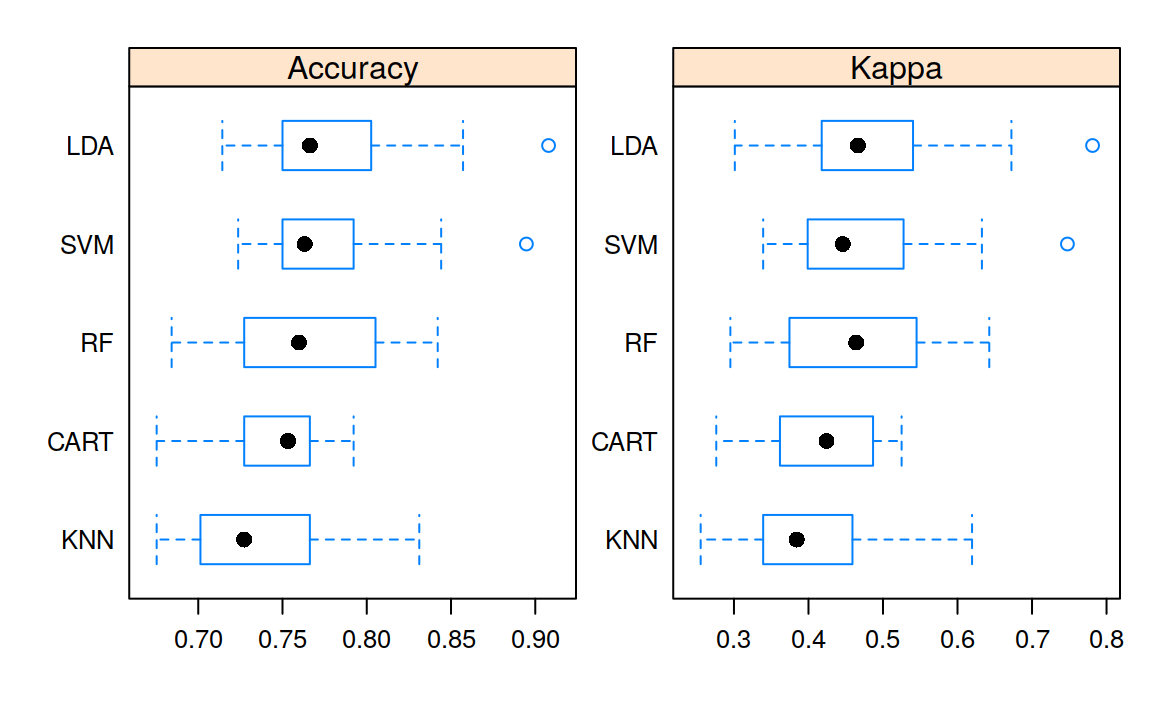
\includegraphics[width=0.7\linewidth]{regression_246-Generalised_Additive_Models-mauna_loa_files/figure-latex/unnamed-chunk-5-1} \end{center}

We can fit a GAM for these data using:

\begin{Shaded}
\begin{Highlighting}[]
\NormalTok{CO2_time <-}\StringTok{ }\KeywordTok{gam}\NormalTok{(co2 }\OperatorTok{~}\StringTok{ }\KeywordTok{s}\NormalTok{(time), }\DataTypeTok{data =}\NormalTok{ CO2, }\DataTypeTok{method =} \StringTok{"REML"}\NormalTok{)}
\end{Highlighting}
\end{Shaded}

which fits a model with a single smooth term for time. We can look at the predicted values for this:

\begin{Shaded}
\begin{Highlighting}[]
\KeywordTok{plot}\NormalTok{(CO2_time)}
\end{Highlighting}
\end{Shaded}

\begin{center}\includegraphics[width=0.7\linewidth]{regression_246-Generalised_Additive_Models-mauna_loa_files/figure-latex/unnamed-chunk-7-1} \end{center}

Note how the smooth term actually reduces to a `normal' linear term here (with an edf of 1) -- that's the nice thing about penalised regression splines. But if we check the model, then we see something is amuck.

\begin{Shaded}
\begin{Highlighting}[]
\KeywordTok{par}\NormalTok{(}\DataTypeTok{mfrow =} \KeywordTok{c}\NormalTok{(}\DecValTok{2}\NormalTok{,}\DecValTok{2}\NormalTok{))}
\KeywordTok{gam.check}\NormalTok{(CO2_time)}
\CommentTok{#> }
\CommentTok{#> Method: REML   Optimizer: outer newton}
\CommentTok{#> full convergence after 8 iterations.}
\CommentTok{#> Gradient range [-0.000145,6.46e-05]}
\CommentTok{#> (score 291 & scale 4.79).}
\CommentTok{#> Hessian positive definite, eigenvalue range [0.000145,65].}
\CommentTok{#> Model rank =  10 / 10 }
\CommentTok{#> }
\CommentTok{#> Basis dimension (k) checking results. Low p-value (k-index<1) may}
\CommentTok{#> indicate that k is too low, especially if edf is close to k'.}
\CommentTok{#> }
\CommentTok{#>         k' edf k-index p-value    }
\CommentTok{#> s(time)  9   1    0.16  <2e-16 ***}
\CommentTok{#> ---}
\CommentTok{#> Signif. codes:  0 '***' 0.001 '**' 0.01 '*' 0.05 '.' 0.1 ' ' 1}
\end{Highlighting}
\end{Shaded}

\begin{center}\includegraphics[width=0.7\linewidth]{regression_246-Generalised_Additive_Models-mauna_loa_files/figure-latex/unnamed-chunk-8-1} \end{center}

The residual plots have a very odd looking rise-and-fall pattern -- clearly there is some dependance structure (and we can probably guess it has something to do with intra-annual fluctuations). Let's try again, and introduce something called a cyclical smoother.

\[ y = \beta_0 + f_{\mathrm{intrannual}}(month) + f_{\mathrm{trend}}(time) + \varepsilon, \quad \varepsilon \sim N(0, \sigma^2)\]

The cyclical smooth term, \(f_{\mathrm{intrannual}}(month)\), is comprised of basis functions just the same as we have seen already, except that the end points of the spline are constrained to be equal -- which makes sense when we're modelling a variable that is cyclical (across months/years).

We'll now see the bs = argument to choose the type of smoother, and the k = argument to choose the number of knots, because cubic regression splines have a set number of knots. We use 12 knots, because there are 12 months.

\begin{Shaded}
\begin{Highlighting}[]
\NormalTok{CO2_season_time <-}\StringTok{ }\KeywordTok{gam}\NormalTok{(co2 }\OperatorTok{~}\StringTok{ }\KeywordTok{s}\NormalTok{(month, }\DataTypeTok{bs =} \StringTok{'cc'}\NormalTok{, }\DataTypeTok{k =} \DecValTok{12}\NormalTok{) }\OperatorTok{+}\StringTok{ }\KeywordTok{s}\NormalTok{(time), }
                       \DataTypeTok{data =}\NormalTok{ CO2, }
                       \DataTypeTok{method =} \StringTok{"REML"}\NormalTok{)}
\end{Highlighting}
\end{Shaded}

Let's look at the fitted smooth terms:

\begin{Shaded}
\begin{Highlighting}[]
\KeywordTok{par}\NormalTok{(}\DataTypeTok{mfrow =} \KeywordTok{c}\NormalTok{(}\DecValTok{1}\NormalTok{,}\DecValTok{2}\NormalTok{))}
\KeywordTok{plot}\NormalTok{(CO2_season_time)}
\end{Highlighting}
\end{Shaded}

\begin{center}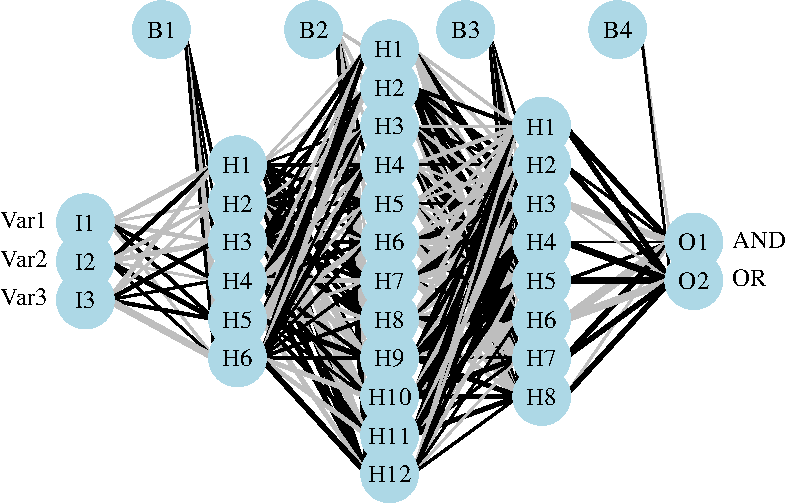
\includegraphics[width=0.7\linewidth]{regression_246-Generalised_Additive_Models-mauna_loa_files/figure-latex/unnamed-chunk-10-1} \end{center}

Looking at both smooth terms, we can see that the monthly smoother is picking up that monthly rise and fall of CO2 -- looking at the relative magnitudes (i.e.~monthly fluctuation vs.~long-term trend), we can see how important it is to disintangle the components of the time series. Let's see how the model diagnostics look now:

\begin{Shaded}
\begin{Highlighting}[]
\KeywordTok{par}\NormalTok{(}\DataTypeTok{mfrow =} \KeywordTok{c}\NormalTok{(}\DecValTok{2}\NormalTok{,}\DecValTok{2}\NormalTok{))}
\KeywordTok{gam.check}\NormalTok{(CO2_season_time)}
\CommentTok{#> }
\CommentTok{#> Method: REML   Optimizer: outer newton}
\CommentTok{#> full convergence after 6 iterations.}
\CommentTok{#> Gradient range [-2.64e-06,5.26e-08]}
\CommentTok{#> (score 87.7 & scale 0.144).}
\CommentTok{#> Hessian positive definite, eigenvalue range [1.03,65.4].}
\CommentTok{#> Model rank =  20 / 20 }
\CommentTok{#> }
\CommentTok{#> Basis dimension (k) checking results. Low p-value (k-index<1) may}
\CommentTok{#> indicate that k is too low, especially if edf is close to k'.}
\CommentTok{#> }
\CommentTok{#>             k'   edf k-index p-value    }
\CommentTok{#> s(month) 10.00  8.67    0.72  <2e-16 ***}
\CommentTok{#> s(time)   9.00  6.61    0.87    0.09 .  }
\CommentTok{#> ---}
\CommentTok{#> Signif. codes:  0 '***' 0.001 '**' 0.01 '*' 0.05 '.' 0.1 ' ' 1}
\end{Highlighting}
\end{Shaded}

\begin{center}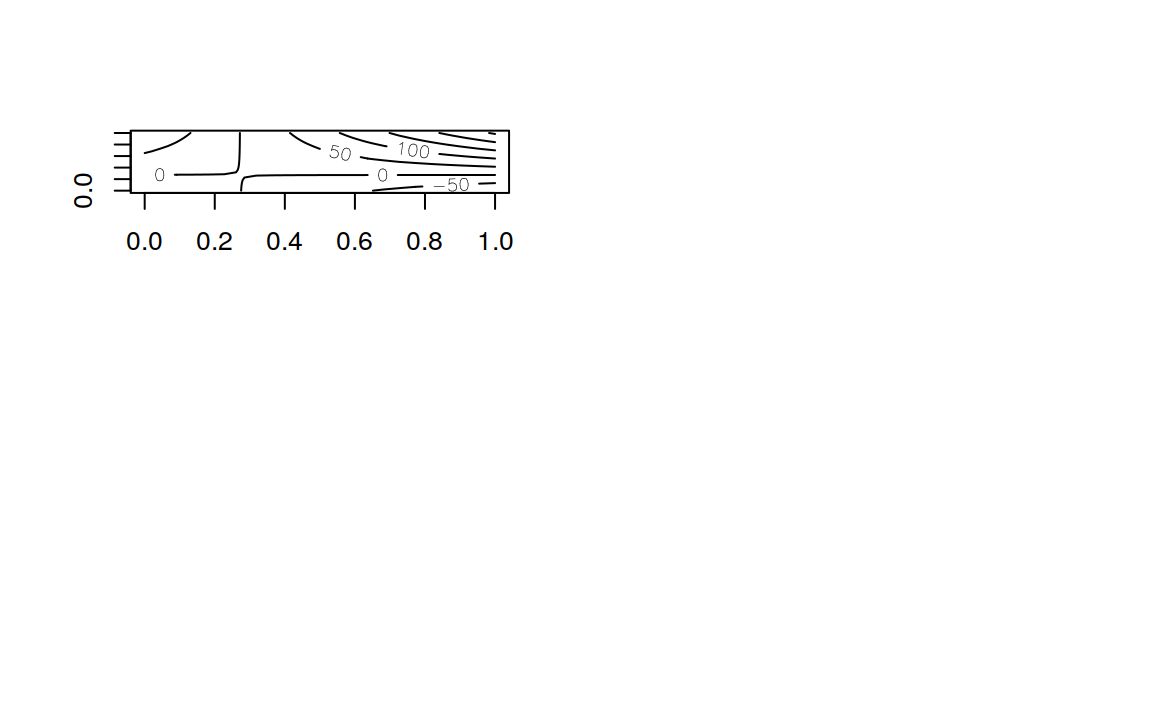
\includegraphics[width=0.7\linewidth]{regression_246-Generalised_Additive_Models-mauna_loa_files/figure-latex/unnamed-chunk-11-1} \end{center}

Much better. Let's look at how the seasonal component stacks up against the full long term trend.

\begin{Shaded}
\begin{Highlighting}[]
\NormalTok{CO2_season_time <-}\StringTok{ }\KeywordTok{gam}\NormalTok{(co2 }\OperatorTok{~}\StringTok{ }\KeywordTok{s}\NormalTok{(month, }\DataTypeTok{bs =} \StringTok{'cc'}\NormalTok{, }\DataTypeTok{k =} \DecValTok{12}\NormalTok{) }\OperatorTok{+}\StringTok{ }\KeywordTok{s}\NormalTok{(time), }
                       \DataTypeTok{data =}\NormalTok{ CO2_dat, }
                       \DataTypeTok{method =} \StringTok{"REML"}\NormalTok{)}
\KeywordTok{par}\NormalTok{(}\DataTypeTok{mfrow =} \KeywordTok{c}\NormalTok{(}\DecValTok{1}\NormalTok{,}\DecValTok{2}\NormalTok{))}
\KeywordTok{plot}\NormalTok{(CO2_season_time)}
\end{Highlighting}
\end{Shaded}

\begin{center}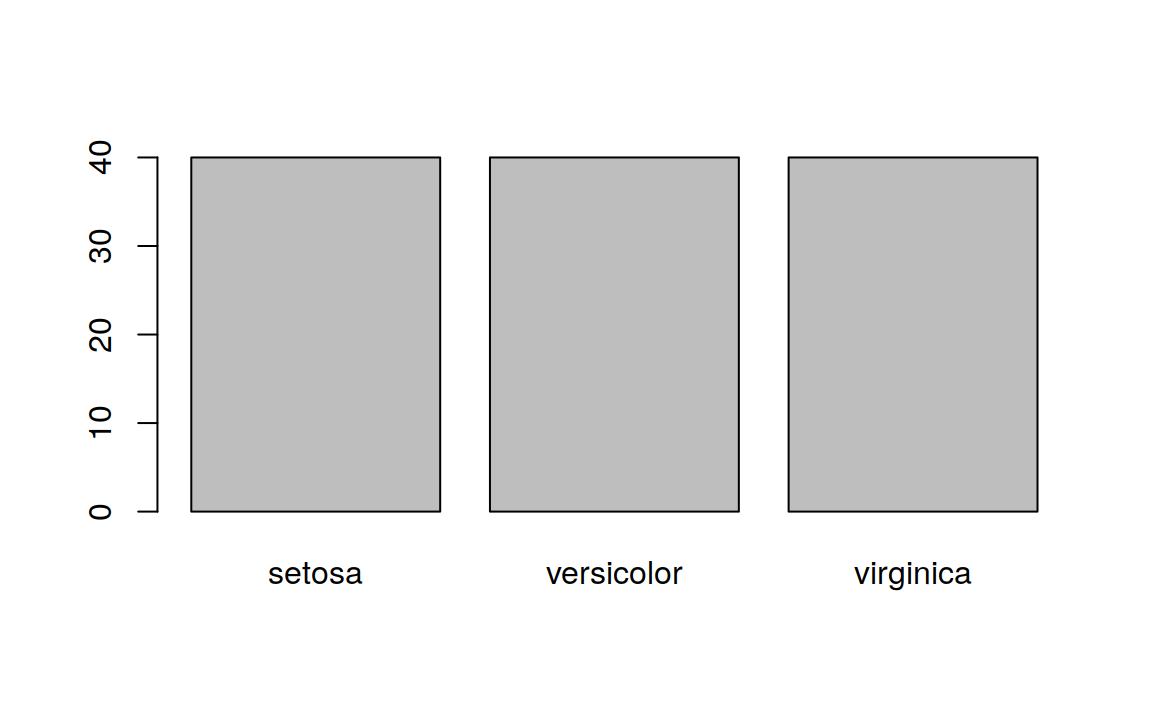
\includegraphics[width=0.7\linewidth]{regression_246-Generalised_Additive_Models-mauna_loa_files/figure-latex/unnamed-chunk-12-1} \end{center}

There's more to the story -- pephaps spatial autocorrelations of some kind? gam can make use of the spatial autocorrelation structures available in the nlme package, more on that next time. Hopefully for the meantime GAMs now don't seem qutie so scary or magical, and you can start to make use of what is really an inrecibly flexible and powerful modelling framework.

\hypertarget{communicating-the-results}{%
\section{Communicating the results}\label{communicating-the-results}}

You can essentially present model results from a GAM as if it were any other linear model, the main difference being that for the smooth terms, there is no single coefficient you can make inference from (i.e.~negative, positive, effect size etc.). So you need to rely on either interpretting the parital effects of the smooth terms visually (e.g.~from a call to plot(gam\_model)) or make inference from the predicted values. You can of course include normal linear terms in the model (either continuous or categorical, and in an ANOVA type framework even) and make inference from them like you normally would. Indeed, GAMs are often useful for accounting for a non-linear phenomonon that is not directly of interest, but needs to be acocunted for when making inferece about other variables.

You can plot the partial effects by calling the plot function on a fitted gam model, and you can look at the parametric terms too, possibly using the termplot function too. You can use ggplot for simple models like we did earlier in this tutorial, but for more complex models, it's good to know how to make the data using predict. We just use the existing time-series here, but you would generate your own data for the \texttt{newdata=} argument.

\begin{Shaded}
\begin{Highlighting}[]
\NormalTok{CO2_pred <-}\StringTok{ }\KeywordTok{data.frame}\NormalTok{(}\DataTypeTok{time =}\NormalTok{ CO2_dat}\OperatorTok{$}\NormalTok{time,}
                       \DataTypeTok{co2 =}\NormalTok{ CO2_dat}\OperatorTok{$}\NormalTok{co2,}
                       \DataTypeTok{predicted_values =} \KeywordTok{predict}\NormalTok{(CO2_season_time, }
                                                  \DataTypeTok{newdata =}\NormalTok{ CO2_dat))}
\KeywordTok{ggplot}\NormalTok{(CO2_pred, }\KeywordTok{aes}\NormalTok{(}\DataTypeTok{x =}\NormalTok{ time)) }\OperatorTok{+}
\StringTok{  }\KeywordTok{geom_point}\NormalTok{(}\KeywordTok{aes}\NormalTok{(}\DataTypeTok{y =}\NormalTok{ co2), }\DataTypeTok{size =} \DecValTok{1}\NormalTok{, }\DataTypeTok{alpha =} \FloatTok{0.5}\NormalTok{) }\OperatorTok{+}\StringTok{ }
\StringTok{    }\KeywordTok{geom_line}\NormalTok{(}\KeywordTok{aes}\NormalTok{(}\DataTypeTok{y =}\NormalTok{ predicted_values), }\DataTypeTok{colour =} \StringTok{"red"}\NormalTok{)}
\end{Highlighting}
\end{Shaded}

\begin{center}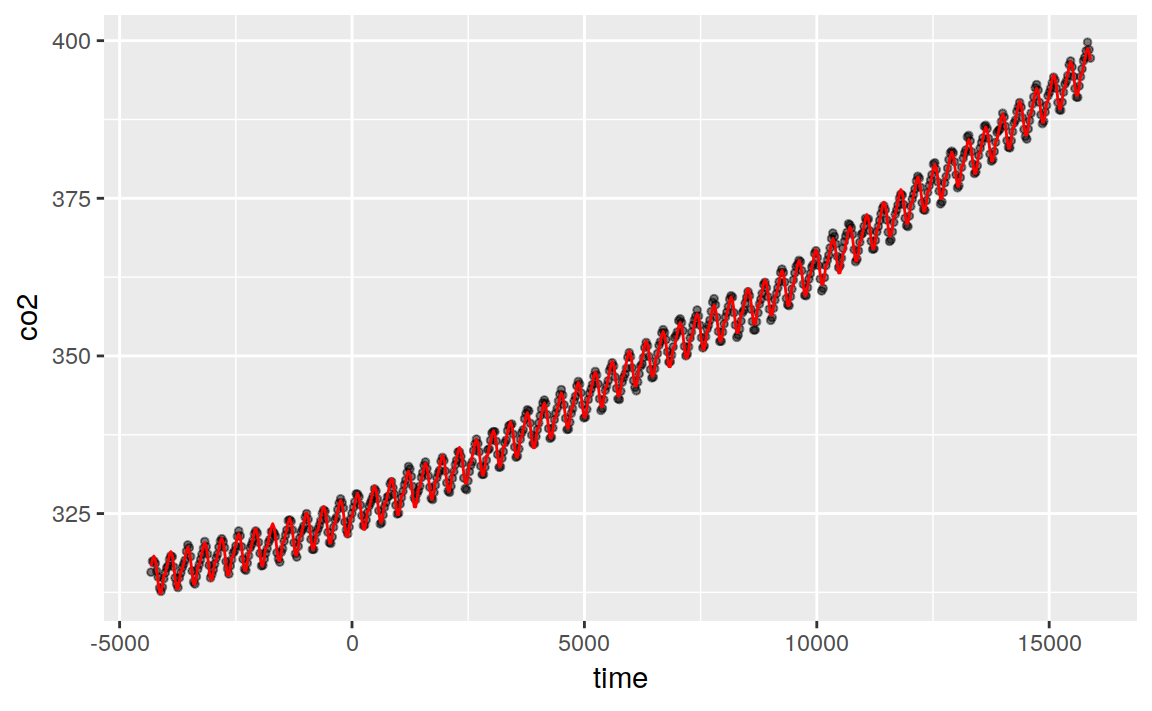
\includegraphics[width=0.7\linewidth]{regression_246-Generalised_Additive_Models-mauna_loa_files/figure-latex/unnamed-chunk-13-1} \end{center}

\hypertarget{fitting-gams-with-brms-part-1}{%
\chapter{Fitting GAMs with brms: part 1}\label{fitting-gams-with-brms-part-1}}

\hypertarget{introduction-1}{%
\section{Introduction}\label{introduction-1}}

Source: \url{https://www.fromthebottomoftheheap.net/2018/04/21/fitting-gams-with-brms/}

Regular readers will know that I have a somewhat unhealthy relationship with GAMs and the \texttt{mgcv} package. I use these models all the time in my research but recently we've been hitting the limits of the range of models that \texttt{mgcv} can fit. So I've been looking into alternative ways to fit the GAMs I want to fit but which can handle the kinds of data or distributions that have been cropping up in our work. The \texttt{brms} package (Bürkner, 2017) is an excellent resource for modellers, providing a high-level R front end to a vast array of model types, all fitted using Stan. \texttt{brms} is the perfect package to go beyond the limits of mgcv because \texttt{brms} even uses the smooth functions provided by \texttt{mgcv}, making the transition easier. In this post I take a look at how to fit a simple GAM in \texttt{brms} and compare it with the same model fitted using \texttt{mgcv}.

\hypertarget{load-packages}{%
\section{Load packages}\label{load-packages}}

In this post we'll use the following packages.

\begin{Shaded}
\begin{Highlighting}[]
\CommentTok{## packages}
\KeywordTok{library}\NormalTok{(mgcv)}
\CommentTok{#> Loading required package: nlme}
\CommentTok{#> This is mgcv 1.8-28. For overview type 'help("mgcv-package")'.}
\KeywordTok{library}\NormalTok{(brms)}
\CommentTok{#> Loading required package: Rcpp}
\CommentTok{#> Registered S3 methods overwritten by 'ggplot2':}
\CommentTok{#>   method         from }
\CommentTok{#>   [.quosures     rlang}
\CommentTok{#>   c.quosures     rlang}
\CommentTok{#>   print.quosures rlang}
\CommentTok{#> Registered S3 method overwritten by 'xts':}
\CommentTok{#>   method     from}
\CommentTok{#>   as.zoo.xts zoo}
\CommentTok{#> Loading 'brms' package (version 2.8.0). Useful instructions}
\CommentTok{#> can be found by typing help('brms'). A more detailed introduction}
\CommentTok{#> to the package is available through vignette('brms_overview').}
\CommentTok{#> }
\CommentTok{#> Attaching package: 'brms'}
\CommentTok{#> The following objects are masked from 'package:mgcv':}
\CommentTok{#> }
\CommentTok{#>     s, t2}
\KeywordTok{library}\NormalTok{(ggplot2)}
\KeywordTok{library}\NormalTok{(schoenberg)}

\KeywordTok{theme_set}\NormalTok{(}\KeywordTok{theme_bw}\NormalTok{())}
\end{Highlighting}
\end{Shaded}

If you don't know \texttt{schoenberg}, it's a package I'm writing to provide \texttt{ggplot} versions of plots that can be produced by \texttt{mgcv} from fitted GAM objects. \texttt{schoenberg} is in early development, but it currently works well enough to plot the models we fit here. If you've never come across this package before, you can install it from Github using \texttt{devtools::install\_github(\textquotesingle{}gavinsimpson/schoenberg}').

\hypertarget{mass-motorcycle-dataset}{%
\section{MASS motorcycle dataset}\label{mass-motorcycle-dataset}}

To illustrate brms's GAM-fitting chops, we'll use the \texttt{mcycle} data set that comes with the \texttt{MASS} package. It contains a set of measurements of the acceleration force on a rider's head during a simulated motorcycle collision and the time, in milliseconds, post collision. The data are loaded using \texttt{data()} and we take a look at the first few rows:

\begin{Shaded}
\begin{Highlighting}[]
\CommentTok{## load the example data mcycle}
\KeywordTok{data}\NormalTok{(mcycle, }\DataTypeTok{package =} \StringTok{'MASS'}\NormalTok{)}

\CommentTok{## show data}
\KeywordTok{head}\NormalTok{(mcycle)}
\CommentTok{#>   times accel}
\CommentTok{#> 1   2.4   0.0}
\CommentTok{#> 2   2.6  -1.3}
\CommentTok{#> 3   3.2  -2.7}
\CommentTok{#> 4   3.6   0.0}
\CommentTok{#> 5   4.0  -2.7}
\CommentTok{#> 6   6.2  -2.7}
\end{Highlighting}
\end{Shaded}

The aim is to model the acceleration force (\texttt{accel}) as a function of time post collision (\texttt{times}). The plot below shows the data.

\begin{Shaded}
\begin{Highlighting}[]
\KeywordTok{ggplot}\NormalTok{(mcycle, }\KeywordTok{aes}\NormalTok{(}\DataTypeTok{x =}\NormalTok{ times, }\DataTypeTok{y =}\NormalTok{ accel)) }\OperatorTok{+}
\StringTok{    }\KeywordTok{geom_point}\NormalTok{() }\OperatorTok{+}
\StringTok{    }\KeywordTok{labs}\NormalTok{(}\DataTypeTok{x =} \StringTok{"Miliseconds post impact"}\NormalTok{, }\DataTypeTok{y =} \StringTok{"Acceleration (g)"}\NormalTok{,}
         \DataTypeTok{title =} \StringTok{"Simulated Motorcycle Accident"}\NormalTok{,}
         \DataTypeTok{subtitle =} \StringTok{"Measurements of head acceleration"}\NormalTok{)}
\end{Highlighting}
\end{Shaded}

\begin{center}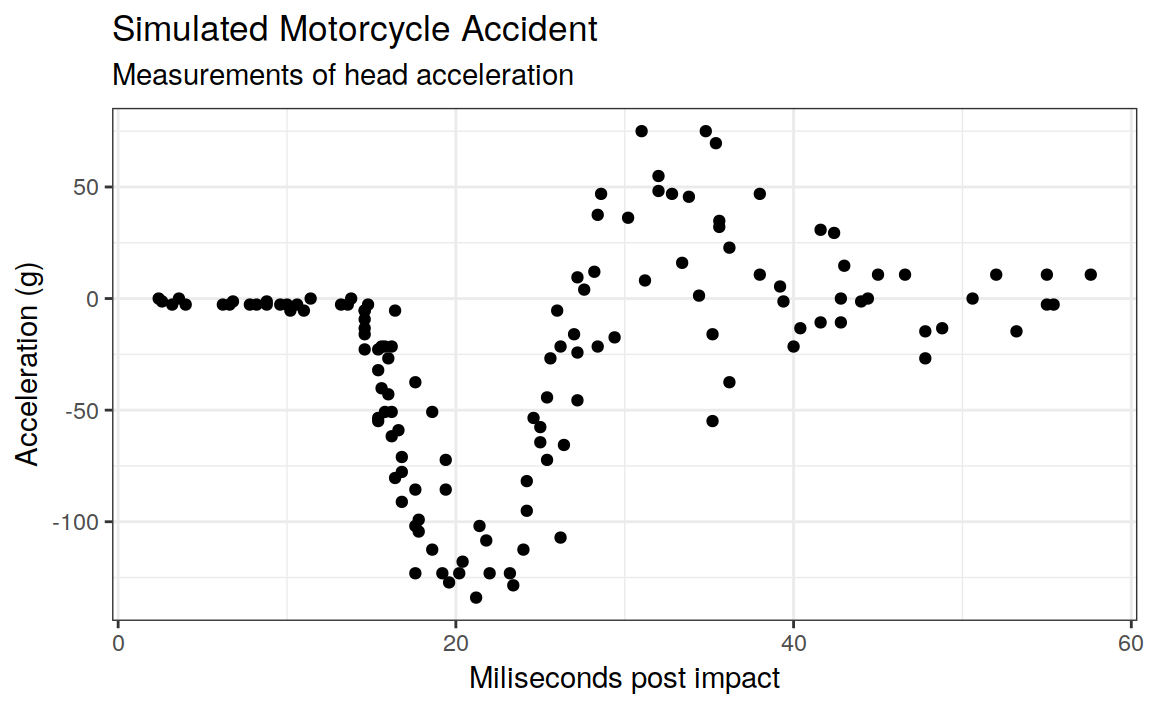
\includegraphics[width=0.7\linewidth]{regression_247-gam_motorcycle_files/figure-latex/unnamed-chunk-4-1} \end{center}

We'll model acceleration as a smooth function of time using a GAM and the default thin plate regression spline basis. This can be done using the \texttt{gam()} function in \texttt{mgcv} and, for comparison with the fully bayesian model we'll fit shortly, we use \texttt{method\ =\ "REML"} to estimate the smoothness parameter for the spline in mixed model form using REML.\\

\begin{Shaded}
\begin{Highlighting}[]
\NormalTok{m1 <-}\StringTok{ }\KeywordTok{gam}\NormalTok{(accel }\OperatorTok{~}\StringTok{ }\KeywordTok{s}\NormalTok{(times), }\DataTypeTok{data =}\NormalTok{ mcycle, }\DataTypeTok{method =} \StringTok{"REML"}\NormalTok{)}
\KeywordTok{summary}\NormalTok{(m1)}
\CommentTok{#> }
\CommentTok{#> Family: gaussian }
\CommentTok{#> Link function: identity }
\CommentTok{#> }
\CommentTok{#> Formula:}
\CommentTok{#> accel ~ s(times)}
\CommentTok{#> }
\CommentTok{#> Parametric coefficients:}
\CommentTok{#>             Estimate Std. Error t value Pr(>|t|)    }
\CommentTok{#> (Intercept)   -25.55       1.95   -13.1   <2e-16 ***}
\CommentTok{#> ---}
\CommentTok{#> Signif. codes:  0 '***' 0.001 '**' 0.01 '*' 0.05 '.' 0.1 ' ' 1}
\CommentTok{#> }
\CommentTok{#> Approximate significance of smooth terms:}
\CommentTok{#>           edf Ref.df    F p-value    }
\CommentTok{#> s(times) 8.62   8.96 53.4  <2e-16 ***}
\CommentTok{#> ---}
\CommentTok{#> Signif. codes:  0 '***' 0.001 '**' 0.01 '*' 0.05 '.' 0.1 ' ' 1}
\CommentTok{#> }
\CommentTok{#> R-sq.(adj) =  0.783   Deviance explained = 79.7%}
\CommentTok{#> -REML = 616.14  Scale est. = 506.35    n = 133}
\end{Highlighting}
\end{Shaded}

As we can see from the model summary, the estimated smooth uses about 8.5 effective degrees of freedom and in the test of zero effect, the null hypothesis is strongly rejected. The fitted spline explains about 80\% of the variance or deviance in the data.

To plot the fitted smooth we could use the \texttt{plot()} method provided by \texttt{mgcv}, but this uses base graphics. Instead we can use the \texttt{draw()} method from \texttt{schoenberg}, which can currently handle most of the univariate smooths in \texttt{mgcv} plus 2-d tensor product smooths

\begin{Shaded}
\begin{Highlighting}[]
\KeywordTok{draw}\NormalTok{(m1)}
\end{Highlighting}
\end{Shaded}

\begin{center}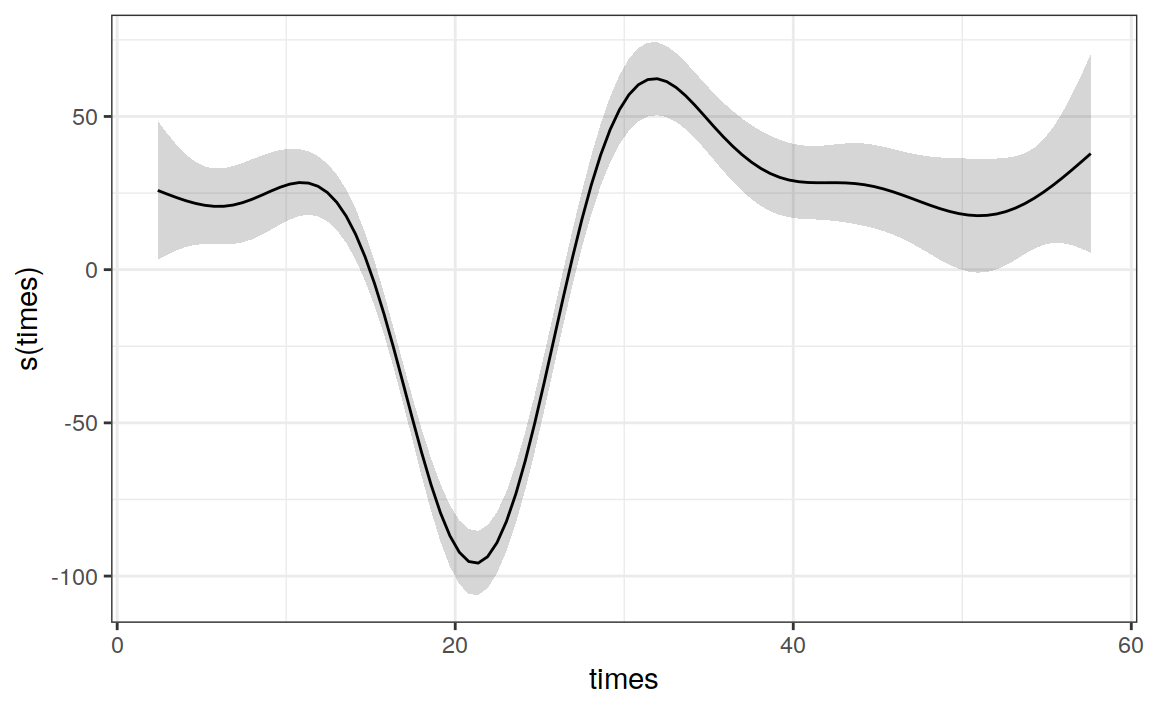
\includegraphics[width=0.7\linewidth]{regression_247-gam_motorcycle_files/figure-latex/draw-1} \end{center}

\hypertarget{bayesian-approach}{%
\section{Bayesian Approach}\label{bayesian-approach}}

The equivalent model can be estimated using a fully-bayesian approach via the \texttt{brm()} function in the \texttt{brms} package. In fact, \texttt{brm()} will use the smooth specification functions from \texttt{mgcv}, making our lives much easier. The major difference though is that you can't use \texttt{te()} or \texttt{ti()} smooths in \texttt{brm()} models; you need to use \texttt{t2()} tensor product smooths instead. This is because the smooths in the model are going to be treated as random effects and the model is estimated as a GLMM, which exploits the duality of splines as random effects. In this representation, the wiggly parts of the spline basis are treated as a random effect and their associated variance parameter controls the degree of wiggliness of the fitted spline. The perfectly smooth parts of the basis are treated as a fixed effect. In this form, the GAM can be estimated using standard GLMM software; it's what allows the \texttt{gamm4()} function to fit GAMMs using the \texttt{lme4} package for example. This is also the reason why we can't use \texttt{te()} or \texttt{ti()} smooths; those smooths do not have nicely separable penalties which means they can't be written in the form required to be fitted using typical mixed model software.

The \texttt{brm()} version of the GAM is fitted using the code below. Note that I have changed a few things from their default values as:

\begin{enumerate}
\def\labelenumi{\arabic{enumi}.}
\item
  the model required more than the default number of MCMC samples - \texttt{iter\ =\ 4000},
\item
  the samples needed thinning to deal with some strong autocorrelation in the Markov chains - \texttt{thin\ =\ 10},
\item
  the \texttt{adapt.delta} parameter, a tuning parameter in the NUTS sampler for Hamiltonian Monte Carlo, potentially needed raising - there was a warning about a potential divergent transition but I should have looked to see if it was one or not; instead I just increased the tuning parameter to \texttt{0.99},
\item
  four chains fitted by default but I wanted these to be fitted using 4 CPU cores,
\item
  \texttt{seed} sets the internal random number generator seed, which allows reproducibility of models, and
\item
  for this post I didn't want to print out the progress of the sampler - \texttt{refresh\ =\ 0} - typically you won't want to do this so you can see how sampling is progressing.
\end{enumerate}

The rest of the model is pretty similar to the \texttt{gam()} version we fitted earlier. The main difference is that I use the \texttt{bf()} function to create a special \texttt{brms} formula specifying the model. You don't actually need to do this for such a simple model, but in a later post we'll use this to fit distributional GAMs. Note that I'm leaving all the priors in the model at the default values. I'll look at defining priors in a later post; for now I'm just going to use the default priors that \texttt{brm()} uses.\\

\begin{Shaded}
\begin{Highlighting}[]
\NormalTok{m2 <-}\StringTok{ }\KeywordTok{brm}\NormalTok{(}\KeywordTok{bf}\NormalTok{(accel }\OperatorTok{~}\StringTok{ }\KeywordTok{s}\NormalTok{(times)),}
          \DataTypeTok{data =}\NormalTok{ mcycle, }\DataTypeTok{family =} \KeywordTok{gaussian}\NormalTok{(), }\DataTypeTok{cores =} \DecValTok{4}\NormalTok{, }\DataTypeTok{seed =} \DecValTok{17}\NormalTok{,}
          \DataTypeTok{iter =} \DecValTok{4000}\NormalTok{, }\DataTypeTok{warmup =} \DecValTok{1000}\NormalTok{, }\DataTypeTok{thin =} \DecValTok{10}\NormalTok{, }\DataTypeTok{refresh =} \DecValTok{0}\NormalTok{,}
          \DataTypeTok{control =} \KeywordTok{list}\NormalTok{(}\DataTypeTok{adapt_delta =} \FloatTok{0.99}\NormalTok{))}
\CommentTok{#> Compiling the C++ model}
\CommentTok{#> Start sampling}
\end{Highlighting}
\end{Shaded}

Once the model has finished compiling and sampling we can output the model summary:\\

\begin{Shaded}
\begin{Highlighting}[]
\KeywordTok{summary}\NormalTok{(m2)}
\CommentTok{#>  Family: gaussian }
\CommentTok{#>   Links: mu = identity; sigma = identity }
\CommentTok{#> Formula: accel ~ s(times) }
\CommentTok{#>    Data: mcycle (Number of observations: 133) }
\CommentTok{#> Samples: 4 chains, each with iter = 4000; warmup = 1000; thin = 10;}
\CommentTok{#>          total post-warmup samples = 1200}
\CommentTok{#> }
\CommentTok{#> Smooth Terms: }
\CommentTok{#>               Estimate Est.Error l-95% CI u-95% CI Eff.Sample Rhat}
\CommentTok{#> sds(stimes_1)   717.02    184.01   460.62  1147.78        991 1.00}
\CommentTok{#> }
\CommentTok{#> Population-Level Effects: }
\CommentTok{#>           Estimate Est.Error l-95% CI u-95% CI Eff.Sample Rhat}
\CommentTok{#> Intercept   -25.52      1.98   -29.38   -21.53       1190 1.00}
\CommentTok{#> stimes_1     17.06     37.98   -59.02    88.95       1144 1.00}
\CommentTok{#> }
\CommentTok{#> Family Specific Parameters: }
\CommentTok{#>       Estimate Est.Error l-95% CI u-95% CI Eff.Sample Rhat}
\CommentTok{#> sigma    22.73      1.53    20.02    26.16       1153 1.00}
\CommentTok{#> }
\CommentTok{#> Samples were drawn using sampling(NUTS). For each parameter, Eff.Sample }
\CommentTok{#> is a crude measure of effective sample size, and Rhat is the potential }
\CommentTok{#> scale reduction factor on split chains (at convergence, Rhat = 1).}
\end{Highlighting}
\end{Shaded}

This output details of the model fitted plus parameter estimates (as posterior means), standard errors, (by default) 95\% credible intervals and two other diagnostics:

\begin{enumerate}
\def\labelenumi{\arabic{enumi}.}
\tightlist
\item
  \texttt{Eff.Sample} is the effective sample size of the posterior samples in the model, and
\item
  \texttt{Rhat} is the potential scale reduction factor or Gelman-Rubin diagnostic and is a measure of how well the chains have converged and ideally should be equal to 1.
\end{enumerate}

The summary includes two entries for the smooth of times:

\begin{enumerate}
\def\labelenumi{\arabic{enumi}.}
\tightlist
\item
  \texttt{sds(stimes\_1)} is the variance parameter, which has the effect of controlling the wiggliness of the smooth - the larger this value the more wiggly the smooth. We can see that the credible interval doesn't include 0 so there is evidence that a smooth is required over and above a linear parametric effect of times, details of which are given next,
\item
  \texttt{stimes\_1} is the fixed effect part of the spline, which is the linear function that is perfectly smooth.
\end{enumerate}

The final parameter table includes information on the variance of the data about the conditional mean of the response.

\hypertarget{comparison}{%
\section{Comparison}\label{comparison}}

\textbf{How does this model compare with the one fitted using gam()?} We can use the \texttt{gam.vcomp()} function to compute the variance component representation of the smooth estimated via \texttt{gam()}. To make it comparable with the value shown for the \texttt{brms} model, we don't undo the rescaling of the penalty matrix that \texttt{gam()} performs to help with numeric stability during model fitting.\\

\begin{Shaded}
\begin{Highlighting}[]
\KeywordTok{gam.vcomp}\NormalTok{(m1, }\DataTypeTok{rescale =} \OtherTok{FALSE}\NormalTok{)}
\CommentTok{#> }
\CommentTok{#> Standard deviations and 0.95 confidence intervals:}
\CommentTok{#> }
\CommentTok{#>          std.dev lower  upper}
\CommentTok{#> s(times)   807.9 480.7 1357.9}
\CommentTok{#> scale       22.5  19.9   25.5}
\CommentTok{#> }
\CommentTok{#> Rank: 2/2}
\end{Highlighting}
\end{Shaded}

This gives a posterior mean of 807.89 with 95\% confidence interval of 480.66--1357.88, which compares well with posterior mean and credible interval of the \texttt{brm()} version of 722.44 (450.17 -- 1150.27).

The \texttt{marginal\_smooths()} function is used to extract the marginal effect of the spline.

This function extracts enough information about the estimated spline to plot it using the \texttt{plot()} method

\begin{Shaded}
\begin{Highlighting}[]
\NormalTok{msms <-}\StringTok{ }\KeywordTok{marginal_smooths}\NormalTok{(m2)}
\KeywordTok{plot}\NormalTok{(msms)}
\end{Highlighting}
\end{Shaded}

\begin{center}\includegraphics[width=0.7\linewidth]{regression_247-gam_motorcycle_files/figure-latex/unnamed-chunk-7-1} \end{center}

Given the similarity in the variance components of the two models it is not surprising the two estimated smooth also look similar. The \texttt{marginal\_smooths()} function is effectively the equivalent of the \texttt{plot()} method for mgcv-based GAMs.

There's a lot that we can and should do to check the model fit. For now, we'll look at two posterior predictive check plots that \texttt{brms}, via the \texttt{bayesplot} package (Gabry and Mahr, 2018), makes very easy to produce using the \texttt{pp\_check()} function.\\

\begin{Shaded}
\begin{Highlighting}[]
\KeywordTok{pp_check}\NormalTok{(m2)}
\CommentTok{#> Using 10 posterior samples for ppc type 'dens_overlay' by default.}
\end{Highlighting}
\end{Shaded}

\begin{center}\includegraphics[width=0.7\linewidth]{regression_247-gam_motorcycle_files/figure-latex/unnamed-chunk-8-1} \end{center}

The default produces a density plot overlay of the original response values (the thick black line) with 10 draws from the posterior distribution of the model. If the model is a good fit to the data, samples of data sampled from it at the observed values of the covariate(s) should be similar to one another.

Another type of posterior predictive check plot is the empirical cumulative distribution function of the observations and random draws from the model posterior, which we can produce with \texttt{type\ =\ "ecdf\_overlay"}.\\

\begin{Shaded}
\begin{Highlighting}[]
\KeywordTok{pp_check}\NormalTok{(m2, }\DataTypeTok{type =} \StringTok{"ecdf_overlay"}\NormalTok{)}
\CommentTok{#> Using 10 posterior samples for ppc type 'ecdf_overlay' by default.}
\end{Highlighting}
\end{Shaded}

\begin{center}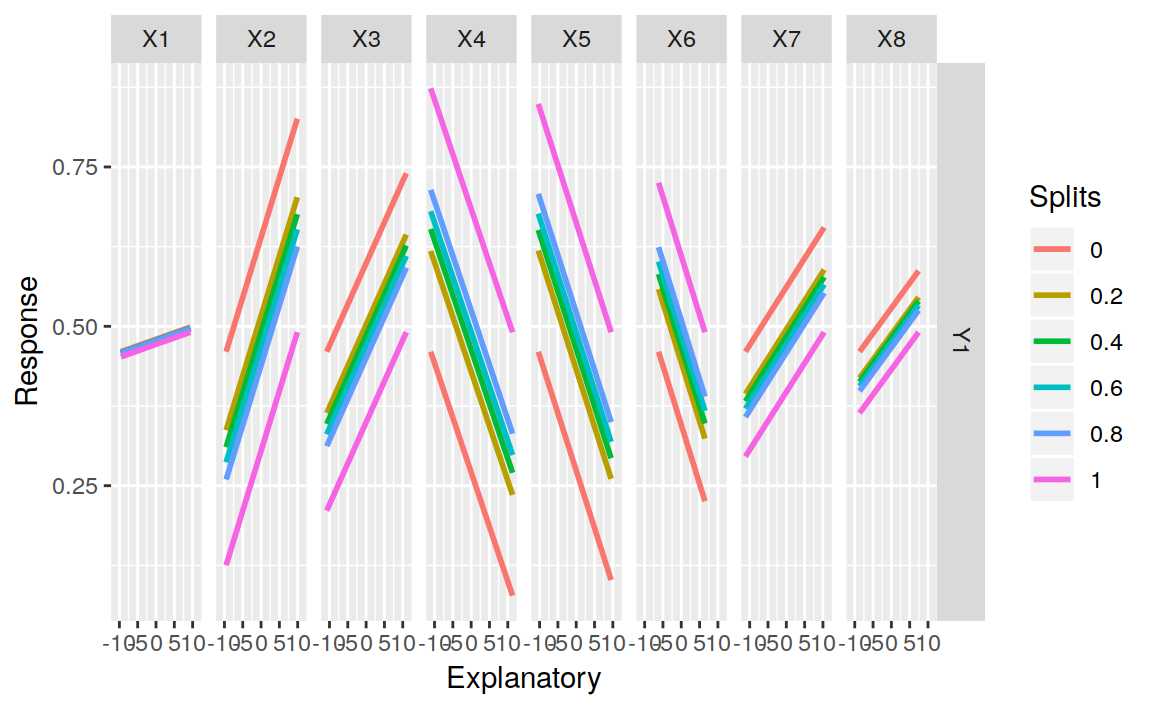
\includegraphics[width=0.7\linewidth]{regression_247-gam_motorcycle_files/figure-latex/unnamed-chunk-9-1} \end{center}

Both plots show significant deviations between the the posterior simulations and the observed data. The poor posterior predictive check results are in large part due to the non-constant variance of the acceleration data conditional upon the covariate. Both models assumed that the observation are distributed Gaussian with means equal to the fitted values (estimated expectation of the response) with the same variance \(\sigma^2\). The observations appear to have different variances, which we can model with a distributional model, which allow all parameters of the distribution of the response to be modelled with linear predictors. We'll take a look at these models in a future post.

\hypertarget{regression-with-stan}{%
\chapter{Regression with Stan}\label{regression-with-stan}}

\url{https://m-clark.github.io/bayesian-basics/models.html}

\hypertarget{regression-models}{%
\section{Regression Models}\label{regression-models}}

Now armed with a conceptual understanding of the Bayesian approach, we will actually investigate a regression model using it. To keep things simple, we start with a standard linear model for regression. Later, we will show how easy it can be to add changes to the sampling distribution or priors for alternative modeling techniques. But before getting too far, you should peruse the Modeling Languages section of the appendix to get a sense of some of the programming approaches available. We will be using the programming language Stan via R and the associated R package \texttt{rstan}. If you prefer to keep things conceptual rather than worry about the code, you can read through the following data description and then skip to running the model.

\hypertarget{example-linear-regression-model}{%
\subsection{Example: Linear Regression Model}\label{example-linear-regression-model}}

In the following we will have some initial data set up and also run the model using the standard lm function for later comparison. I choose simulated data so that not only should you know what to expect from the model, it can easily be modified to enable further understanding. I will also use some matrix operations, and if these techniques are unfamiliar to you, you'll perhaps want to do some refreshing or learning on your own beforehand.

\hypertarget{setup}{%
\subsection{Setup}\label{setup}}

First we need to create the data we'll use here and for most of the other examples in this document. I use simulated data so that there is no ambiguity about what to expect.

\begin{Shaded}
\begin{Highlighting}[]
\KeywordTok{library}\NormalTok{(rstan)}
\CommentTok{#> Loading required package: ggplot2}
\CommentTok{#> Registered S3 methods overwritten by 'ggplot2':}
\CommentTok{#>   method         from }
\CommentTok{#>   [.quosures     rlang}
\CommentTok{#>   c.quosures     rlang}
\CommentTok{#>   print.quosures rlang}
\CommentTok{#> Loading required package: StanHeaders}
\CommentTok{#> rstan (Version 2.18.2, GitRev: 2e1f913d3ca3)}
\CommentTok{#> For execution on a local, multicore CPU with excess RAM we recommend calling}
\CommentTok{#> options(mc.cores = parallel::detectCores()).}
\CommentTok{#> To avoid recompilation of unchanged Stan programs, we recommend calling}
\CommentTok{#> rstan_options(auto_write = TRUE)}
\KeywordTok{library}\NormalTok{(rstanarm)}
\CommentTok{#> Loading required package: Rcpp}
\CommentTok{#> Registered S3 method overwritten by 'xts':}
\CommentTok{#>   method     from}
\CommentTok{#>   as.zoo.xts zoo}
\CommentTok{#> rstanarm (Version 2.18.2, packaged: 2018-11-08 22:19:38 UTC)}
\CommentTok{#> - Do not expect the default priors to remain the same in future rstanarm versions.}
\CommentTok{#> Thus, R scripts should specify priors explicitly, even if they are just the defaults.}
\CommentTok{#> - For execution on a local, multicore CPU with excess RAM we recommend calling}
\CommentTok{#> options(mc.cores = parallel::detectCores())}
\CommentTok{#> - Plotting theme set to bayesplot::theme_default().}
\CommentTok{#> }
\CommentTok{#> Attaching package: 'rstanarm'}
\CommentTok{#> The following object is masked from 'package:rstan':}
\CommentTok{#> }
\CommentTok{#>     loo}
\KeywordTok{library}\NormalTok{(dplyr)}
\CommentTok{#> }
\CommentTok{#> Attaching package: 'dplyr'}
\CommentTok{#> The following objects are masked from 'package:stats':}
\CommentTok{#> }
\CommentTok{#>     filter, lag}
\CommentTok{#> The following objects are masked from 'package:base':}
\CommentTok{#> }
\CommentTok{#>     intersect, setdiff, setequal, union}

\KeywordTok{rstan_options}\NormalTok{(}\DataTypeTok{auto_write =} \OtherTok{TRUE}\NormalTok{)}
\KeywordTok{options}\NormalTok{(}\DataTypeTok{mc.cores =}\NormalTok{ parallel}\OperatorTok{::}\KeywordTok{detectCores}\NormalTok{())}
\end{Highlighting}
\end{Shaded}

\begin{Shaded}
\begin{Highlighting}[]
\CommentTok{# set seed for replicability}
\KeywordTok{set.seed}\NormalTok{(}\DecValTok{8675309}\NormalTok{)}

\CommentTok{# create a N x k matrix of covariates}
\NormalTok{N =}\StringTok{ }\DecValTok{250}
\NormalTok{K =}\StringTok{ }\DecValTok{3}

\NormalTok{covariates =}\StringTok{ }\KeywordTok{replicate}\NormalTok{(K, }\KeywordTok{rnorm}\NormalTok{(}\DataTypeTok{n=}\NormalTok{N))}
\KeywordTok{colnames}\NormalTok{(covariates) =}\StringTok{ }\KeywordTok{c}\NormalTok{(}\StringTok{'X1'}\NormalTok{, }\StringTok{'X2'}\NormalTok{, }\StringTok{'X3'}\NormalTok{)}

\CommentTok{# create the model matrix with intercept}
\NormalTok{X =}\StringTok{ }\KeywordTok{cbind}\NormalTok{(}\DataTypeTok{Intercept=}\DecValTok{1}\NormalTok{, covariates)}
\KeywordTok{glimpse}\NormalTok{(X)}
\CommentTok{#>  num [1:250, 1:4] 1 1 1 1 1 1 1 1 1 1 ...}
\CommentTok{#>  - attr(*, "dimnames")=List of 2}
\CommentTok{#>   ..$ : NULL}
\CommentTok{#>   ..$ : chr [1:4] "Intercept" "X1" "X2" "X3"}
\KeywordTok{head}\NormalTok{(X)}
\CommentTok{#>      Intercept     X1     X2     X3}
\CommentTok{#> [1,]         1 -0.997 -0.333 -0.391}
\CommentTok{#> [2,]         1  0.722 -0.174  2.213}
\CommentTok{#> [3,]         1 -0.617 -0.187 -1.563}
\CommentTok{#> [4,]         1  2.029  1.156 -0.770}
\CommentTok{#> [5,]         1  1.065 -0.938 -0.555}
\CommentTok{#> [6,]         1  0.987  0.524  1.411}
\end{Highlighting}
\end{Shaded}

\begin{Shaded}
\begin{Highlighting}[]
\CommentTok{# create a normally distributed variable that is a function of the covariates}
\NormalTok{coefs =}\StringTok{ }\KeywordTok{c}\NormalTok{(}\DecValTok{5}\NormalTok{, }\FloatTok{.2}\NormalTok{, }\FloatTok{-1.5}\NormalTok{, }\FloatTok{.9}\NormalTok{)}
\NormalTok{mu =}\StringTok{ }\NormalTok{X }\OperatorTok\StringTok{ }\NormalTok{coefs}
\KeywordTok{glimpse}\NormalTok{(mu)}
\CommentTok{#>  num [1:250, 1] 4.95 7.4 3.75 2.98 6.12 ...}
\end{Highlighting}
\end{Shaded}

\begin{Shaded}
\begin{Highlighting}[]
\CommentTok{# same as}
\CommentTok{# y = 5 + .2*X1 - 1.5*X2 + .9*X3 + rnorm(N, mean=0, sd=2)}

\NormalTok{sigma =}\StringTok{ }\DecValTok{2}
\NormalTok{y =}\StringTok{ }\KeywordTok{rnorm}\NormalTok{(N, mu, sigma)}
\KeywordTok{glimpse}\NormalTok{(y)}
\CommentTok{#>  num [1:250] 5.21 9.76 3.71 3.7 2.92 ...}
\end{Highlighting}
\end{Shaded}

Just to make sure we're on the same page, at this point we have three covariates, and a \(y\) that is a normally distributed, linear function of them, and with standard deviation equal to 2. The population values for the coefficients including the intercept are 5, 0.2, -1.5, and 0.9, though with the noise added, the actual estimated values for the sample are slightly different. Now we are ready to set up an R list object of the data for input into Stan, as well as the corresponding Stan code to model this data. I will show all the Stan code, which is implemented in R via a single character string, and then provide some detail on each corresponding model block. However, the goal here isn't to focus on tools as it is to focus on concepts. Related code for this same model in BUGS and JAGS is provided in the appendix here. I don't think there is an easy way to learn these programming languages except by diving in and using them yourself with models and data you understand.

\begin{Shaded}
\begin{Highlighting}[]
\CommentTok{# Run lm for later comparison; but go ahead and examine now if desired}
\NormalTok{modlm =}\StringTok{ }\KeywordTok{lm}\NormalTok{(y}\OperatorTok{~}\NormalTok{., }\DataTypeTok{data=}\KeywordTok{data.frame}\NormalTok{(X[,}\OperatorTok{-}\DecValTok{1}\NormalTok{]))}
\KeywordTok{summary}\NormalTok{(modlm)}
\CommentTok{#> }
\CommentTok{#> Call:}
\CommentTok{#> lm(formula = y ~ ., data = data.frame(X[, -1]))}
\CommentTok{#> }
\CommentTok{#> Residuals:}
\CommentTok{#>    Min     1Q Median     3Q    Max }
\CommentTok{#> -6.863 -1.470  0.243  1.421  5.041 }
\CommentTok{#> }
\CommentTok{#> Coefficients:}
\CommentTok{#>             Estimate Std. Error t value Pr(>|t|)    }
\CommentTok{#> (Intercept)   4.8978     0.1284   38.13  < 2e-16 ***}
\CommentTok{#> X1            0.0841     0.1296    0.65     0.52    }
\CommentTok{#> X2           -1.4686     0.1261  -11.64  < 2e-16 ***}
\CommentTok{#> X3            0.8196     0.1207    6.79  8.2e-11 ***}
\CommentTok{#> ---}
\CommentTok{#> Signif. codes:  0 '***' 0.001 '**' 0.01 '*' 0.05 '.' 0.1 ' ' 1}
\CommentTok{#> }
\CommentTok{#> Residual standard error: 2.02 on 246 degrees of freedom}
\CommentTok{#> Multiple R-squared:  0.452,  Adjusted R-squared:  0.446 }
\CommentTok{#> F-statistic: 67.8 on 3 and 246 DF,  p-value: <2e-16}
\end{Highlighting}
\end{Shaded}

The data list for Stan should include any matrix, vector, or value that might be used in the Stan code. For example, along with the data one can include things like sample size, group indicators (e.g.~for mixed models) and so forth. Here we can get by with just the sample size (N), the number of columns in the model matrix (K), the target variable (y) and the model matrix itself (X).

\begin{Shaded}
\begin{Highlighting}[]
\CommentTok{# Create the data list object for Stan input}
\NormalTok{dat =}\StringTok{ }\KeywordTok{list}\NormalTok{(}\DataTypeTok{N=}\NormalTok{N, }\DataTypeTok{K=}\KeywordTok{ncol}\NormalTok{(X), }\DataTypeTok{y=}\NormalTok{y, }\DataTypeTok{X=}\NormalTok{X)}
\end{Highlighting}
\end{Shaded}

Next comes the Stan code. In \texttt{R2OpenBugs} or \texttt{rjags} one would call a separate text file with the code, and one can do the same with rstan, but for our purposes, we'll display it within the R code. The first thing to note then is the model code. Next, Stan has programming blocks that have to be called in order. I will have all of the blocks in the code to note their order and discuss each in turn, even though we won't use them all. Anything following a \texttt{//} or \texttt{\#}, or between \texttt{/*\ */}, are comments pertaining to the code. Assignments in Stan are \texttt{=}, while distributions are specified with a \texttt{\textasciitilde{}} , e.g. \texttt{y\ \textasciitilde{}\ normal(0,\ 1)} means y is normally distributed with mean 0 and standard deviation of 1.

The primary goal here is to get to the results and beyond, but one should examine the Stan manual for details about the code. In addition, to install rstan one will need to do so via CRAN or GitHub (quickstart guide). It does not require a separate installation of Stan itself, but it does take a couple steps and does require a C++ compiler. Once you have rstan installed it is called like any other R package as will see shortly.

\begin{Shaded}
\begin{Highlighting}[]
\CommentTok{# Create the stan model object using Stan's syntax}
\NormalTok{stanmodelcode =}\StringTok{ "}
\StringTok{data \{                      // Data block}
\StringTok{  int<lower=1> N;           // Sample size}
\StringTok{  int<lower=1> K;           // Dimension of model matrix}
\StringTok{  matrix[N, K] X;           // Model Matrix}
\StringTok{  vector[N] y;              // Target variable}
\StringTok{\}}

\StringTok{/* }
\StringTok{transformed data \{          // Transformed data block. Not used presently.}
\StringTok{\} }
\StringTok{*/}

\StringTok{parameters \{                // Parameters block}
\StringTok{  vector[K] beta;           // Coefficient vector}
\StringTok{  real<lower=0> sigma;      // Error scale}
\StringTok{\}}

\StringTok{model \{                     // Model block}
\StringTok{  vector[N] mu;}
\StringTok{  mu = X * beta;            // Creation of linear predictor}
\StringTok{  }
\StringTok{  // priors}
\StringTok{  beta  ~ normal(0, 10);}
\StringTok{  sigma ~ cauchy(0, 5);     // With sigma bounded at 0, this is half-cauchy}
\StringTok{  }
\StringTok{  // likelihood}
\StringTok{  y ~ normal(mu, sigma);}
\StringTok{\}}

\StringTok{/*}
\StringTok{generated quantities \{      // Generated quantities block. Not used presently.}
\StringTok{\}}
\StringTok{*/}
\StringTok{"}
\end{Highlighting}
\end{Shaded}

\hypertarget{stan-code}{%
\section{Stan Code}\label{stan-code}}

The first section is the data block, where we tell Stan the data it should be expecting from the data list. It is useful to put in bounds as a check on the data input, and that is what is being done between the \texttt{\textless{}\ \textgreater{}} (e.g.~we should at least have a sample size of 1). The first two variables declared are N and K, both as integers. Next the code declares the model matrix and target vector respectively. As you'll note here and for the next blocks, we declare the type and dimensions of the variable and then its name. In Stan, everything declared in one block is available to subsequent blocks, but those declared in a block may not be used in earlier blocks. Even within a block, anything declared, such as N and K, can then be used subsequently, as we did to specify dimensions of the model matrix X.

For a reference, the following is from the Stan manual, and notes variables of interest and the associated blocks where they would be declared.

The transformed data block is where you could do such things as log or center variables and similar, i.e.~you can create new data based on the input data or just in general. If you are using R though, it would almost always be easier to do those things in R first and just include them in the data list. You can also declare any unmodeled parameters here, e.g.~those you want fixed at some value.

The primary parameters of interest that are to be estimated go in the parameters block. As with the data block you can only declare these variables, you cannot make any assignments. Here we note the \(\beta\) and \(\sigma\) to be estimated, with a lower bound of zero on the latter. In practice, you might prefer to split out the intercept or other coefficients to be modeled separately if they are on notably different scales.

The transformed parameters block is where optional parameters of interest might be included. What might go here is fairly open, but for efficiency's sake you will typically want to put things only of specific interest that are dependent on the parameters block. These are evaluated along with the parameters, so if the objects are not of special interest you can instead generate them in the model or generated quantities block to save time.

The model block is where your priors and likelihood are specified, along with the declaration of any variables necessary. As an example, the linear predictor is included here, as it will go towards the likelihood. Note that we could have instead put the linear predictor in the transformed parameters section, but this would slow down the process, and again, we're not so interested in those specific values.

I use a normal prior for the coefficients with a zero mean and a very large standard deviation to reflect my notable ignorance here. For the\\
\(\sigma\) estimate I use a Cauchy distribution. Many regression examples using BUGS will use an inverse gamma prior, which is perfectly okay for this model, though it would not work so well for other variance parameters. Had we not specified anything for the prior distribution for the parameters, vague (discussed more in the Choice of Prior section), uniform distributions would be the default. The likelihood is specified in a similar manner as one would with R. BUGS style languages would actually use \texttt{dnorm} as in R, though Stan uses normal for the function name.

Finally, we get to the generated quantities, which is kind of a fun zone. Anything you want to calculate can go here - predictions on new data, ratios of parameters, how many times a parameter is greater than \texttt{x}, transformations of parameters for reporting purposes, and so forth. We will demonstrate this later.

\hypertarget{running-the-model}{%
\section{Running the Model}\label{running-the-model}}

Now that we have an idea of what the code is doing, let's put it to work. Bayesian estimation, like maximum likelihood, starts with initial guesses as starting points and then runs in an iterative fashion, producing simulated draws from the posterior distribution at each step, and then correcting those draws until finally getting to some target, or stationary distribution. This part is key and different from classical statistics. We are aiming for a distribution, not a point estimate.

The simulation process is referred to as Markov Chain Monte Carlo, or MCMC for short. The specifics of this process are what sets many of the Bayesian programming languages/approaches apart, and something we will cover in more detail in a later section (see Sampling Procedure). In MCMC, all of the simulated draws from the posterior are based on and correlated with previous draws, as the process moves along the path toward a stationary distribution. We will typically allow the process to warm up, or rather get a bit settled down from the initial starting point, which might be way off, and thus the subsequent estimates will also be way off for the first few iterations. Rest assured, assuming the model and data are otherwise acceptable, the process will get to where it needs to go. However, as a further check, we will run the whole thing multiple times, i.e.~have more than one chain. As the chains will start from different places, if multiple chains get to the same place in the end, we can feel more confident about our results.

While this process may sound like it might take a long time to complete, for the following you'll note that it will likely take more time for Stan to compile its code to C++ than it will to run the model, and on my computer each chain only takes only a little more than a second. However, the Bayesian approach used to take a very long time even for a standard regression such as this, and that is perhaps the primary reason why Bayesian analysis only caught on in the last couple decades; we simply didn't have the machines to do it efficiently. Even now though, for highly complex models and large data sets it can still take a long time to run, though typically not prohibitively so.

In the following code, we note the object that contains the Stan model code, the data list, how many iterations we want (5000), how long we want the process to run before we start to keep any estimates (\texttt{warmup=2500}), how many of the post-warmup draws of the posterior we want to keep (\texttt{thin=10} means every tenth draw), and the number of chains (\texttt{chains=4}). In the end, we will have four chains of 100028 draws from the posterior distribution of the parameters. Stan spits out a lot of output to the R console even with \texttt{verbose\ =\ FALSE}, and I omit it here, but you will see some initial info about the compiling process, updates as each chain gets through 10\% of iterations specified in the iter argument, and finally an estimate of the elapsed time. You may also see informational messages which, unless they are highly repetitive, should not be taken as an error.

\begin{Shaded}
\begin{Highlighting}[]
\KeywordTok{library}\NormalTok{(rstan)}

\CommentTok{### Run the model and examine results}
\NormalTok{fit =}\StringTok{ }\KeywordTok{stan}\NormalTok{(}\DataTypeTok{model_code =}\NormalTok{ stanmodelcode,}
           \DataTypeTok{data =}\NormalTok{ dat,}
           \DataTypeTok{iter =} \DecValTok{5000}\NormalTok{,}
           \DataTypeTok{warmup =} \DecValTok{2500}\NormalTok{,}
           \DataTypeTok{thin =} \DecValTok{10}\NormalTok{,}
           \DataTypeTok{chains =} \DecValTok{4}\NormalTok{)}
\end{Highlighting}
\end{Shaded}

With the model run, we can now examine the results. In the following, we specify the digit precision to display, which parameters we want (not necessary here), and which quantiles of the posterior draws we want, which in this case are the median and those that would produce a 95\% interval estimate.

\begin{Shaded}
\begin{Highlighting}[]
\CommentTok{# summary}
\KeywordTok{print}\NormalTok{(fit, }\DataTypeTok{pars=}\KeywordTok{c}\NormalTok{(}\StringTok{'beta'}\NormalTok{, }\StringTok{'sigma'}\NormalTok{), }\DataTypeTok{digits=}\DecValTok{3}\NormalTok{, }\DataTypeTok{prob=}\KeywordTok{c}\NormalTok{(.}\DecValTok{025}\NormalTok{,.}\DecValTok{5}\NormalTok{,.}\DecValTok{975}\NormalTok{))}
\CommentTok{#> Inference for Stan model: 207e716b728c6bce448b2aa8a19bbe44.}
\CommentTok{#> 4 chains, each with iter=5000; warmup=2500; thin=10; }
\CommentTok{#> post-warmup draws per chain=250, total post-warmup draws=1000.}
\CommentTok{#> }
\CommentTok{#>           mean se_mean    sd   2.5%    50%  97.5% n_eff Rhat}
\CommentTok{#> beta[1]  4.894   0.005 0.130  4.642  4.890  5.134   713    1}
\CommentTok{#> beta[2]  0.086   0.004 0.132 -0.169  0.081  0.336   996    1}
\CommentTok{#> beta[3] -1.463   0.004 0.122 -1.703 -1.466 -1.232   955    1}
\CommentTok{#> beta[4]  0.822   0.004 0.124  0.584  0.822  1.069  1038    1}
\CommentTok{#> sigma    2.034   0.003 0.092  1.858  2.033  2.211   960    1}
\CommentTok{#> }
\CommentTok{#> Samples were drawn using NUTS(diag_e) at Wed Sep 18 14:39:40 2019.}
\CommentTok{#> For each parameter, n_eff is a crude measure of effective sample size,}
\CommentTok{#> and Rhat is the potential scale reduction factor on split chains (at }
\CommentTok{#> convergence, Rhat=1).}
\end{Highlighting}
\end{Shaded}

So far so good. The mean estimates reflect the mean of posterior draws for the parameters of interest, and are the \textbf{typical coefficients} reported in standard regression analysis. The 95\% probability, or, credible intervals are worth noting, because they are not confidence intervals as you know them. There is no repeated sampling interpretation here. The probability interval is more intuitive. It means simply that, based on the results of this model, there is a 95\% chance the true value will fall between those two points. The other values printed out I will return to in just a moment.

Comparing the results to those from R's \texttt{lm} function, we can see we obtain similar estimates, as they are identical to two decimal places. In fact, had we used uniform priors, we would be doing essentially the same model as what is being conducted with standard maximum likelihood estimation. Here, we have a decent amount of data for a model that isn't complex, so we would expect the likelihood to notably outweigh the prior, as we demonstrated previously with our binomial example.

\begin{Shaded}
\begin{Highlighting}[]
\KeywordTok{summary}\NormalTok{(modlm)}
\CommentTok{#> }
\CommentTok{#> Call:}
\CommentTok{#> lm(formula = y ~ ., data = data.frame(X[, -1]))}
\CommentTok{#> }
\CommentTok{#> Residuals:}
\CommentTok{#>    Min     1Q Median     3Q    Max }
\CommentTok{#> -6.863 -1.470  0.243  1.421  5.041 }
\CommentTok{#> }
\CommentTok{#> Coefficients:}
\CommentTok{#>             Estimate Std. Error t value Pr(>|t|)    }
\CommentTok{#> (Intercept)   4.8978     0.1284   38.13  < 2e-16 ***}
\CommentTok{#> X1            0.0841     0.1296    0.65     0.52    }
\CommentTok{#> X2           -1.4686     0.1261  -11.64  < 2e-16 ***}
\CommentTok{#> X3            0.8196     0.1207    6.79  8.2e-11 ***}
\CommentTok{#> ---}
\CommentTok{#> Signif. codes:  0 '***' 0.001 '**' 0.01 '*' 0.05 '.' 0.1 ' ' 1}
\CommentTok{#> }
\CommentTok{#> Residual standard error: 2.02 on 246 degrees of freedom}
\CommentTok{#> Multiple R-squared:  0.452,  Adjusted R-squared:  0.446 }
\CommentTok{#> F-statistic: 67.8 on 3 and 246 DF,  p-value: <2e-16}
\end{Highlighting}
\end{Shaded}

But how would we know if our model was working out okay otherwise? There are several standard diagnostics, and we will talk about them in more detail in the next section, but let's take a look at some presently. In the summary, \texttt{se\_mean} is the Monte Carlo error, and is an estimate of the uncertainty contributed by only having a finite number of posterior draws. \texttt{n\_eff} is effective sample size given all chains, and essentially accounts for autocorrelation in the chain, i.e.~the correlation of the estimates as we go from one draw to the next. It actually doesn't have to be very large, but if it was small relative to the total number of draws desired that might be cause for concern. \texttt{Rhat} is a measure of how well chains mix, and goes to 1 as chains are allowed to run for an infinite number of draws. In this case, \texttt{n\_eff} and \texttt{Rhat} suggest we have good convergence, but we can also examine this visually with a traceplot.

\begin{Shaded}
\begin{Highlighting}[]
\CommentTok{# Visualize}
\KeywordTok{stan_trace}\NormalTok{(fit, }\DataTypeTok{pars=}\KeywordTok{c}\NormalTok{(}\StringTok{'beta[4]'}\NormalTok{))}
\end{Highlighting}
\end{Shaded}

\begin{center}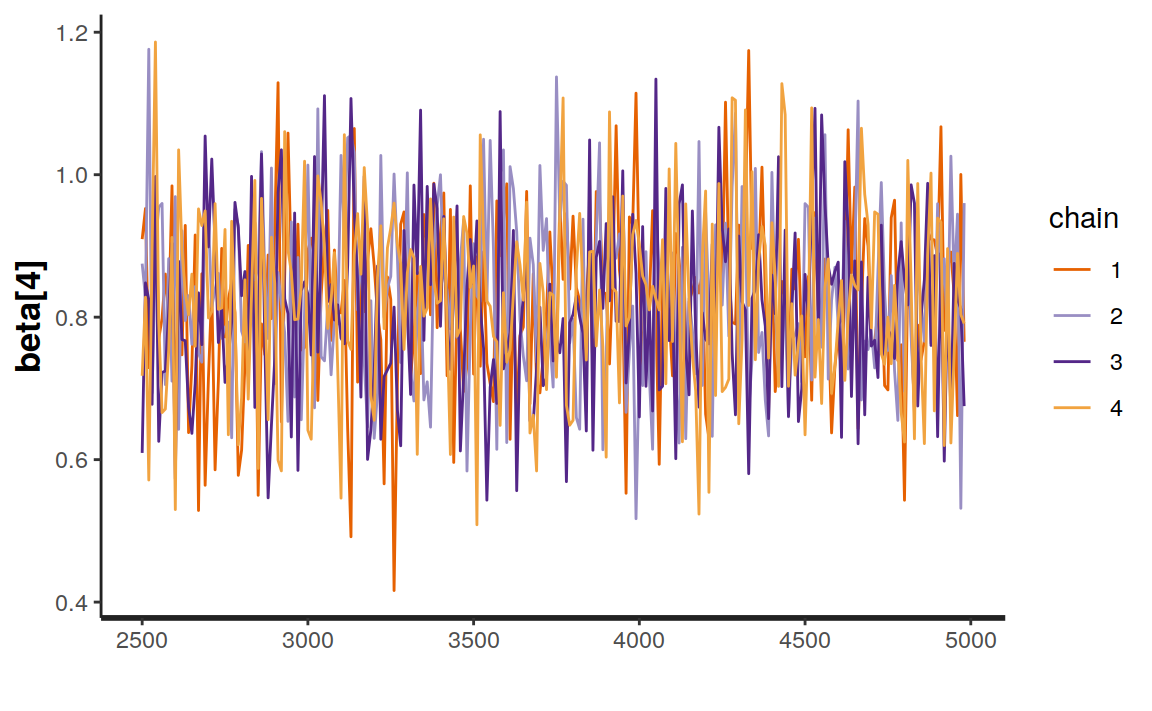
\includegraphics[width=0.7\linewidth]{regression_248-linear_regression_with_stan_files/figure-latex/traceplot-1} \end{center}

I only show one parameter for the current demonstration, but one should always look at the traceplots for all parameters. What we are looking for after the warmup period is a ``fat hairy caterpillar'' or something that might be labeled as ``grassy'', and this plot qualifies as such. One can see that the estimates from each chain find their way from the starting point to a more or less steady state quite rapidly (initial warmup iterations in gray). Furthermore, all three chains, each noted by a different color, are mixing well and bouncing around the same conclusion. The statistical measures and traceplot suggest that we are doing okay.

The Stan development crew has made it easy to interactively explore diagnostics via the \texttt{shinystan} package, and one should do so with each model. In addition, there are other diagnostics available in the coda package, and Stan model results can be easily converted to work with it. The following code demonstrates how to get started.

\begin{Shaded}
\begin{Highlighting}[]
\KeywordTok{library}\NormalTok{(coda)}
\CommentTok{#> }
\CommentTok{#> Attaching package: 'coda'}
\CommentTok{#> The following object is masked from 'package:rstan':}
\CommentTok{#> }
\CommentTok{#>     traceplot}
\NormalTok{betas =}\StringTok{ }\KeywordTok{extract}\NormalTok{(fit, }\DataTypeTok{pars=}\StringTok{'beta'}\NormalTok{)}\OperatorTok{$}\NormalTok{beta}
\NormalTok{betas.mcmc =}\StringTok{ }\KeywordTok{as.mcmc}\NormalTok{(betas)}
\CommentTok{# plot(betas.mcmc)}
\end{Highlighting}
\end{Shaded}

\begin{Shaded}
\begin{Highlighting}[]
\ControlFlowTok{if}\NormalTok{ (}\KeywordTok{interactive}\NormalTok{()) }\KeywordTok{launch_shinystan}\NormalTok{(fit)}
\end{Highlighting}
\end{Shaded}

So there you have it. Aside from the initial setup with making a data list and producing the language-specific model code, it doesn't necessarily take much to running a Bayesian regression model relative to standard models. The main thing perhaps is simply employing a different mindset, and interpreting the results from within that new perspective. For the standard models you are familiar with, it probably won't take too long to be as comfortable here as you were with those, and now you will have a flexible tool to take you into new realms with deeper understanding.

\bibliography{book.bib,packages.bib}


\end{document}
